%! Author = Lennart Kloock

\documentclass[11pt]{article}
\usepackage{geometry}
\usepackage{graphicx}
\usepackage{wrapfig}
\usepackage{tocloft}
\usepackage[ngerman]{babel}
\usepackage[utf8]{inputenc}
\usepackage{amsmath}
\usepackage{hyphenat}
\usepackage[bottom]{footmisc}
\usepackage[backend=biber,citestyle=authortitle]{biblatex}
\usepackage{csquotes}
\usepackage{subcaption}
\usepackage[
    hidelinks,
    pdfauthor={Lennart Kloock},
    pdftitle={Theorie kuenstlicher neuronaler Netze und Anwendung am Beispiel von Bilderkennung}
]{hyperref}
\usepackage{amssymb}
\usepackage{lipsum}

\addbibresource{quellen.bib}
\geometry{a4paper, left=4cm, right=2cm, top=2cm, bottom=2cm}
\renewcommand{\baselinestretch}{1.5}
\hyphenation{Mathe-matik wieder-gewinnen}
\makeatletter\newcommand{\lofwithouttitle}{\@starttoc{lof}}\makeatother

% Um die Nummern im Literaturverzeichnis zu verstecken.
\DeclareFieldFormat{labelnumberwidth}{}
\setlength{\biblabelsep}{0pt}

\begin{document}

    \pagenumbering{gobble}
    \begin{titlepage}
        \begin{center}
            \vspace*{1cm}
            \Huge
            \textbf{Theorie künstlicher neuronaler Netze und Anwendung am Beispiel von Bilderkennung}\\

            \vspace{0.5cm}
            \LARGE
            Facharbeit im Rahmen des Mathematikunterrichts\\

            \vspace{1.5cm}
            \textbf{Lennart Kloock}\\

            \vfill
            \large
            Albert-Schweitzer-Gymnasium Hürth\\
            Fachlehrerin: Frau Marschner\\

            \vspace{0.5cm}
            Eingereicht am 29.~März~2021
        \end{center}
    \end{titlepage}

    \tableofcontents
    \pagebreak

    \pagenumbering{arabic}
    \setcounter{page}{3}

    \section{Einleitung}\label{sec:einleitung}
Der Mensch ist sehr gut darin Objekte, Motive und Zeichen zu erkennen, die auf einem Bild abgebildet sind.
Das menschliche Gehirn kann dabei auch Bildern die gleiche Bezeichnung zuordnen, die sich von allen anderen Bildern unterscheiden, die es jemals gesehen hat.
Beispielsweise können Menschen eine fremde Handschrift lesen, obwohl sie diese zuvor noch nie gesehen haben.
Ein Computer kann dagegen nur festen Programmabläufen folgen und ist allein mit vorbestimmten Algorithmen nicht in der Lage, unbekannte Daten zu analysieren und zu interpretieren.
Künstliche neuronale Netze versuchen, dem Computer das Prinzip des Lernens beizubringen.
Auf dieses Prinzip wird in dieser Arbeit eingegangen, indem erst der Aufbau und die Funktionsweise eines solchen künstlichen neuronalen Netzes erklärt werden.
Anschließend geht es um die dadurch gewonnene Lernfähigkeit und dessen Anwendung.
Das Ziel dieser Arbeit ist es, die Theorie und Anwendung von einfachen künstlichen neuronalen Netzen zu erklären und an einem Beispiel der Bilderkennung zu zeigen.\\
Künstliche Intelligenz ist für die meisten Menschen schon ein Teil ihres Alltags geworden, ohne dass sie es gemerkt haben.
Von der Autokorrektur der Handytastatur bis hin zu Sprach-, Bild- und Gesichtserkennung funktioniert heutzutage vieles mit künstlicher Intelligenz und künstlichen neuronalen Netzen.
Inzwischen setzen viele Menschen auf die Technik, die durch die neuronalen Netze ermöglicht wird.
Diese vielen verschiedenen Anwendungsmöglichkeiten und deren mathematischer Hintergrund sind der Grund für mein Interesse an diesem Thema.

    \section{Die Geschichte künstlicher neuronaler Netze}\label{sec:die-geschichte}
Die Forschung an künstlichen neuronalen Netzen hatte bereits in den 1940er Jahren ihre Anfänge und wurde durch viele verschiedene Wissenschaftler betrieben.\\
1943 veröffentlichten \textsc{Warren~McCulloch} und \textsc{Walter~Pitts} eine Arbeit\footcite{mcculloch} in der sie behaupteten, dass die von ihnen beschriebenen Netze so gut wie jede gesuchte Funktion berechnen könnten.
Kurz danach nannten sie eine mögliche Anwendungsmöglichkeit im Gebiet der Erkennung von räumlichen Mustern.\\
In den Jahren nach der Veröffentlichung \textsc{McCulloch} und \textsc{Pitts}’ Arbeit wurde viel an den Netzen geforscht und auch verändert.
Unter anderem wurde 1949 vom Psychologen \textsc{Donald~O.~Hebb} die klassische \textit{Hebb'sche~Lernregel} aufgestellt.
Diese Regel gilt als Grundlage für die meisten anderen Lernregeln und ist nicht nur auf künstliche neuronale Netze anwendbar.\\
\textsc{Frank~Rosenblatt} und \textsc{Charles~Wightman} begannen 1957 am MIT mit der Entwicklung des \textit{Perceptron}s, ein einfaches neuronales Netzwerk, das sie in Form des Neurocomputers \textit{Mark~I~Perceptron} implementierten.
Der \textit{Mark~I~Perceptron} konnte bereits eine Ziffer in einem $20 \times 20$ Pixel Bild erkennen.\\
1960 entwarfen \textsc{Bernard~Widrow} und \textsc{Marcian~E.~Hoff} die \textit{Deltaregel} beziehungsweise den \textit{LMS-Algorithmus}, mit dem das ebenfalls von \textsc{Widrow} und \textsc{Hoff} entworfene \textit{ADALINE}~(\textit{Adaptive~Linear~Neuron}) arbeitete.
Es ist ein System, das bereits kommerziell als Echo-Unterdrückung in Analogtelefonen eingesetzt wurde.\\
Als 1969 \textsc{Marvin~Minsky} und \textsc{Seymour~Papert} eine mathematische Analyse des \textit{Perceptron}s veröffentlichten, kam die Forschung im Bereich der künstlichen Intelligenz vollständig zum Erliegen.
Sie hatten in ihrem Buch über \textsc{Frank~Rosenblatt}s einfaches \textit{Perceptron}-Modell einige schwerwiegende Mängel festgestellt, woraufhin viele Forschungsgelder gestrichen wurden.
Wegen der knappen Gelder wurde nur noch wenig am Thema weitergeforscht, was \textsc{Paul Werbos} 1974 dazu veranlasste, das schon vorher bestehende \textit{Backpropagation~of~Error}-Lernverfahren auf neuronale Netze anzuwenden.
Dieses Verfahren wurde jedoch erst 10 Jahre nach seiner Veröffentlichung so wichtig, dass es an weiterer Aufmerksamkeit gewann.\\
Ab den 1980er Jahren nahm der amerikanische Wissenschaftler \textsc{John~Hopfield} sehr viel Einfluss auf das mathematisch-informatisch geprägte Thema, unter anderem indem er 1982 seine \textit{Hopfieldnetze} vorstellte.
Die \textit{Hopfieldnetze} sind eine Art von neuronalen Netzen, die sich an den Gesetzen des Magnetismus in der Physik orientieren.
Außerdem veröffentlicht \textsc{Hopfield} 1985 einen Artikel, in dem er eine Lösung des \textit{Travelling~Salesman~Problem}s mithilfe seiner \textit{Hopfieldnetze} beschreibt.
\textsc{Minsky}s Vorhersagen von 1969 stellten sich als größenteils falsch heraus und das Thema gewann die anfängliche Aufmerksamkeit zurück.\\
Von 1980 bis heute hat sich das Thema der künstlichen Intelligenz rasant weiterentwickelt und ist heute bedeutsamer als je zuvor.
~\footcite[][Abschnitt 1.2]{kriesel}
    \pagebreak

    \section{Aufbau und Funktionsweise eines künstlichen neuronalen Netzes}\label{sec:aufbau}
Dieser Abschnitt geht auf den Aufbau und die Arbeitsweise eines künstlichen neuronalen Netzes (im Folgenden KNN) ein.

\subsection{Neuronale Netze des Gehirns}\label{subsec:gehirn}
Die KNN sind, wie ihr Name schon sagt, inspiriert von den biologischen neuronalen Netzen des Gehirns.
Sie sind ein Versuch, diese biologischen Netze auf Basis von Gehirnforschung zu imitieren.
Das Gehirn besteht unter anderem aus sogenannten Nervenzellen und deren Verbindungen untereinander.
Jede Nervenzelle hat mehrere Tausend dieser Verbindungen, welche auch Synapsen genannt werden.
Die Kommunikation über die Synapsen funktioniert in der Regel mithilfe chemischer Neurotransmitter, die als Botenstoffe zwischen zwei Nervenzellen fungieren.
Bestimmte Nervenzellen können mehr oder weniger Einfluss auf eine andere Zelle nehmen, je nachdem wie nah die verbindende Synapse am Zellkörper der Zelle ansetzt.
Die neuronalen Netze passen sich fortlaufend an ihre Einflüsse (zum Beispiel visuelle oder akustische) an.\\
Die Architektur der künstlichen Netze ist eine stark vereinfachte Form der hier beschriebenen biologisch-chemischen Netze im Gehirn.
~\footcite{ct-netzgespinste}

\subsection{Künstliche Neuronen}\label{subsec:neuronen}
Die Neuronen im Sinne der KNN sind gegenüber den biologischen Neuronen so weit vereinfacht, dass sie nur noch einen Zahlenwert speichern.
Sie stellen die kleinste Einheit eines KNN dar und repräsentieren einen Wert, der entweder direkt aus einem Datensatz kommt~(zum Beispiel die Graustufe eines Pixels) oder aus einer Berechnung auf Basis der Werte von anderen Neuronen (siehe~\autoref{subsec:feedforward}).
~\footcite{3b1b-1}

\subsection{Ebenen}\label{subsec:ebenen}
Die Neuronen der KNN liegen aber nicht, wie im Gehirn, unsortiert vor, sondern sind in Ebenen (engl.~\textit{layers}) angeordnet.
Ein KNN kann beliebig viele Ebenen von je beliebig vielen Neuronen haben.
Das ist unter anderem der Grund für die große Anpassbarkeit der Netzwerke.
Eingabeneuronen heißen die Neuronen, die sich in der ersten Ebene eines KNN befinden und deren Werte die Eingabedaten repräsentieren.
Die Neuronen, die sich auf der letzten Ebene des Netzes befinden, heißen Ausgabeneuronen und repräsentieren die Ausgabe eines Netzes.
Außerdem können die künstlichen Netze Ebenen an Neuronen beinhalten, die weder aus Eingabeneuronen noch aus Ausgabeneuron bestehen.
Eine solche Ebene wird verdeckte Ebene~(engl.~\textit{hidden~layer}) genannt.
Während im Gehirn theoretisch jedes Neuron mit beliebig vielen anderen Neuronen verbunden sein kann, kann ein künstliches Neuron nur mit denen der benachbarten Ebenen verbunden sein.
~\footcite{3b1b-1}

\subsection{Gewichtungen}\label{subsec:gewichtungen}
Die Verbindungen zwischen den künstlichen Neuronen heißen Gewichtungen (engl.~\textit{weights}) und stehen repräsentativ für die Synapsen im Gehirn.
Jedes Neuron ist durch eine Gewichtung mit allen Neuronen der vorherigen und nachfolgenden Ebene verbunden.
Aber auch die Gewichtungen wurden gegenüber den Synapsen stark vereinfacht und auf ihre wichtigste Eigenschaft reduziert.
Der Wert des Neurons, von welchem die Gewichtung ausgeht, wird gewichtet an das Neuron, mit dem die Gewichtung verbunden ist, weitergereicht.
Der Faktor mit dem der eingehende Wert gewichtet wird, ist veränderbar und eine der wichtigsten anpassbaren Faktoren für den Lernprozess (siehe~\autoref{sec:training}).
~\footcite{3b1b-1}

\subsection{Das Feedforward-Verfahren}\label{subsec:feedforward}
Das Weiterverarbeiten einer Menge an Eingabewerten zu einer Menge an Ausgabewerten wird Feedforward (dt.~\textit{Vorwärtskopplung} oder \textit{Vorsteuerung}) genannt.\\
Für ein KNN mit $N^l$ vielen Neuronen auf Ebene $l$ sei $z^l_n$ der Wert des $n$-ten Neurons auf Ebene $l$.
Der Faktor der Gewichtung, die das $n$-te Neuron auf Ebene $l$ mit dem $p$-ten Neuron auf Ebene $l-1$ verbindet, heißt $w^l_{n p}$.
Alle Gewichtungen eines KNN seien definiert durch $\overline{w} = (w^2_{11}, w^2_{12}, w^2_{21}, \dots)$.
Die Werte der Neuronen der ersten Ebene werden nun bis zur letzten Ebene an Neuronen durchgegeben und dabei folgendermaßen verändert:
\begin{itemize}
    \item Der Wert eines Neurons entspricht immer der Summe an gewichteten Werten der Neuronen der vorherigen Ebene.
    \item Ein Wert eines Neurons wird gewichtet, indem er mit dem Faktor der Gewichtung multipliziert wird.
\end{itemize}
Daraus resultiert folgende von $\overline{w}$ abhängige Funktion, die im weiteren Verlauf dieser Arbeit noch ergänzt und abgewandelt werden wird.
\begin{equation}
    z^l_n = \sum\limits^{N^{l-1}}_{i=1} z^{l-1}_i \cdot w^l_{n i}
    \label{eq:z}
\end{equation}
Mit diesem Ausdruck kann nun jeder Wert jedes Neurons berechnet werden.
Zuerst wird der Ausdruck auf die Neuronen der zweiten Ebene angewendet, welche die gewichteten Eingabedaten der ersten Ebene benutzen.
Nachdem die Werte für die zweite Ebene feststehen, können die der dritten Ebene berechnet werden und so weiter.
Nach Anwendung des Feedforward-Verfahrens sind die Werte der letzten Ebene die Ausgabedaten, die das Netz für die Eingabedaten in der ersten Ebene errechnet hat.
~\footcite{3b1b-1}

\subsection{Die Aktivierungsfunktion}\label{subsec:aktivierung}
Doch allein Ebenen von Neuronen und Gewichtungen reichen nicht, damit ein KNN funktioniert.
Um einen ungünstigen Einfluss extremer Werte zu vermeiden, müssen diese normalisiert werden.
Diese Normalisierung wird Aktivierung genannt und wird mit einer sogenannten Aktivierungsfunktion umgesetzt.
In der Regel versucht eine Aktivierungsfunktion den Wert eines Neurons auf einen Bereich zu begrenzen, zum Beispiel mittels stauchen.
\begin{wrapfigure}{r}{0.45\textwidth}
    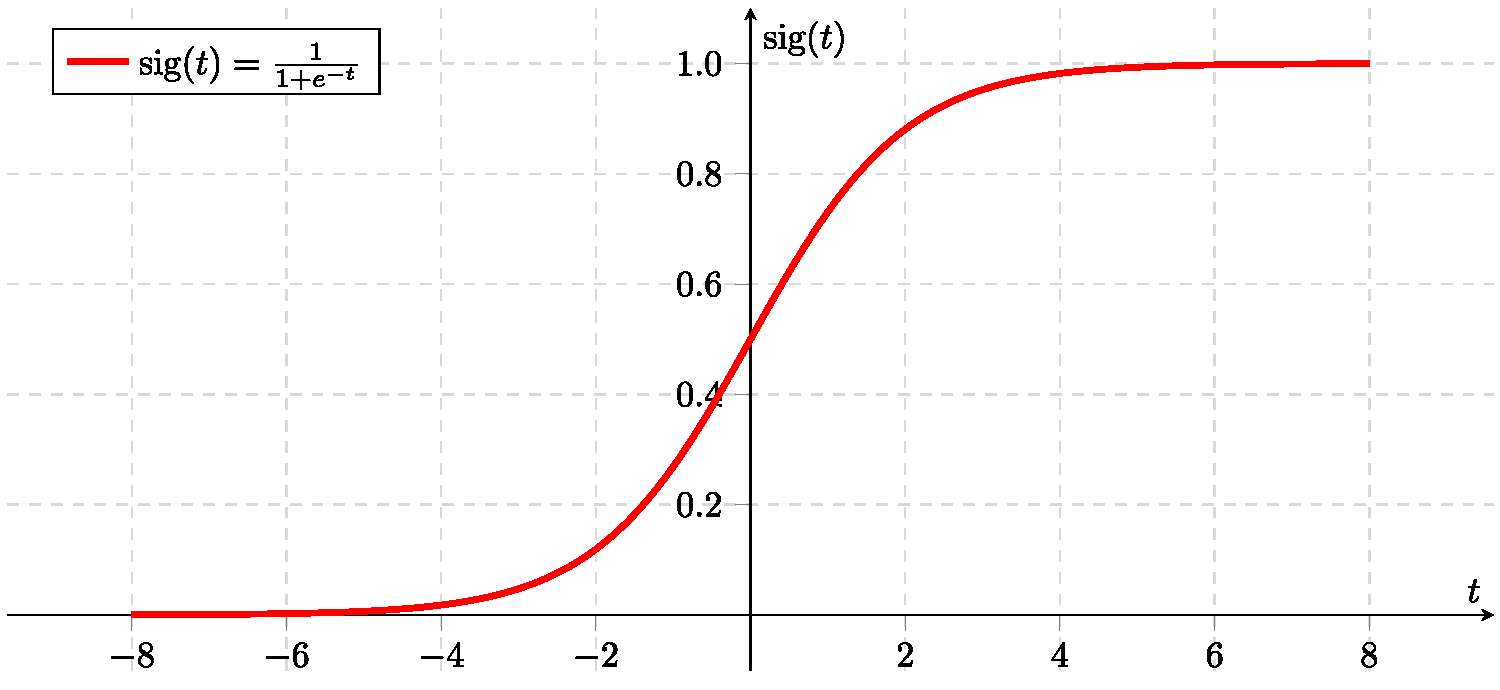
\includegraphics[width=0.45\textwidth]{grafiken/sigmoid}
    \caption[Die logistische Kurve: \textit{Von Martin Thoma, CC0}]{Die logistische Kurve}
    \label{fig:sigmoid}
\end{wrapfigure}
Es gibt mehrere Funktionen die dafür infrage kommen, aber die klassische Funktion um diesen Effekt zu erzielen ist die logistische Funktion $sig$ (\autoref{fig:sigmoid}).
Diese Sigmoidfunktion staucht Werte in den Bereich zwischen 0 und 1, indem die Werte für $t \to -\infty$ gegen 0 laufen und für $t \to \infty$ gegen 1 laufen.
Dazwischen verläuft der Graph der Funktion S-förmig.
Die Funktion wird durch folgenden Term beschrieben.
\begin{equation*}
    sig(t) = \frac{1}{1+e^{-t}}
\end{equation*}
Für die Aktivierungsfunktion $\varphi$ gilt im weiteren Verlauf dieser Arbeit immer $\varphi = sig$.\\
Die Aktivierungsfunktion wird auf den Wert eines Neurons (definiert durch~\eqref{eq:z}) angewendet.
Daraus ergibt sich folgende Funktion für den aktivierten Wert $a^l_n$ des $n$-ten Neurons auf Ebene $l$.
\begin{equation}
    a^l_n = \varphi(z^l_n)
    \label{eq:a}
\end{equation}
Der aktivierte Wert $a^l_n$ wird nun bei Anwendung des Feedforward-Verfahrens anstatt der gewichteten Summe $z^l_n$ genutzt.
Deshalb ändert sich~\eqref{eq:z} nun zu folgendem Ausdruck.
~\footcite{3b1b-1}
\begin{equation}
    z^l_n = \sum\limits^{N^{l-1}}_{i=1} a^{l-1}_i w^l_{n i}
    \label{eq:z-mit-a}
\end{equation}

\subsection{Biases}\label{subsec:biases}
Auch wenn Neuronen, Gewichtungen und eine Aktivierungsfunktion schon reichen damit ein KNN funktioniert, braucht es in den meisten Fällen noch mehr Variabilität.
Aus diesem Grund gibt es den sogenannten Bias (dt.~\textit{Verzerrung} oder \textit{Voreingenommenheit}).
Auch dieser besteht aus einem veränderbaren Zahlenwert, der für jedes Neuron in einem Netz unterschiedlich sein kann.
Ein Bias kann direkten Einfluss auf die Bedeutung seines Neurons nehmen, indem es den Wert direkt erhöht oder erniedrigt.
Dies macht das Netz anpassungsfähiger, was beim Trainieren (siehe \autoref{sec:training}) des Netzes helfen kann.
Falls sich das Neuron, zu dem der Bias gehört, nicht in der ersten Ebene des KNN befindet, wird sein Wert auf den bisherigen Wert des Neurons addiert.
Neuronen auf der ersten Ebene besitzen keine Biases, da sie die originalen Eingabewerte nur verfälschen würden und dadurch zu ungenaueren Ergebnissen beitragen würden.\\
$b^l_n$ entspricht dem Bias des $n$-ten Neurons auf Ebene $l > 1$.
Außerdem werden die Funktionen aus~\eqref{eq:z} und~\eqref{eq:a} erneut leicht angepasst und sind dadurch nun abhängig von $\overline{b}$, was alle Biases eines Netzes repräsentiert und definiert ist durch $\overline{b} = (b^2_1, b^2_2, \dots)$.
~\footcite{3b1b-1}
\begin{align}
    z^l_n &= b^l_n + \sum\limits^{N^{l-1}}_{i=1}a^{l-1}_i w^l_{n i}
    \label{eq:z-neu}\\
    a^l_n &= \varphi(z^l_n)
    \label{eq:a-neu}
\end{align}

\subsection{Beispiel}\label{subsec:beispiel}
\begin{wrapfigure}{r}{0.4\textwidth}
    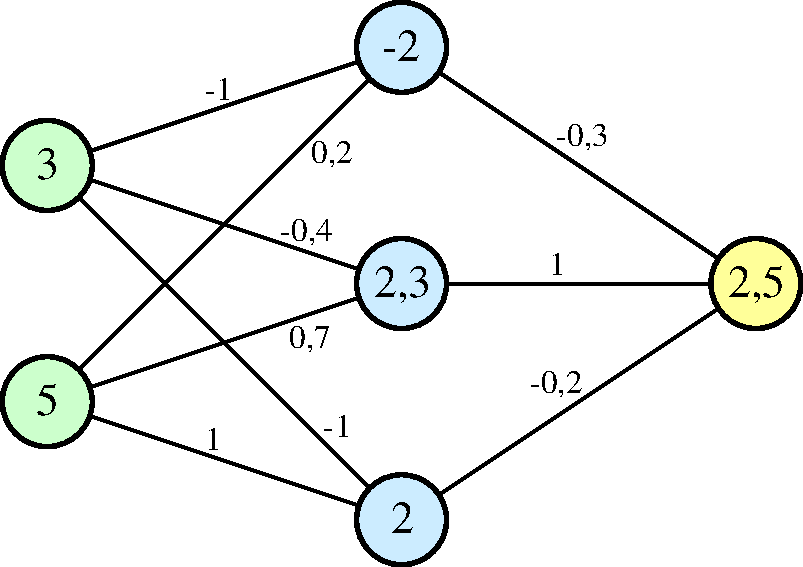
\includegraphics[width=0.4\textwidth]{grafiken/netzwerk_beispiel}
    \caption[Vereinfachte Darstellung eines künstlichen neuronalen Netzes: \textit{Eigene Grafik, erstellt in Inkscape}]{Vereinfachte Darstellung eines künstlichen neuronalen Netzes}
    \label{fig:beispiel_netz}
\end{wrapfigure}
\autoref{fig:beispiel_netz} zeigt ein Beispiel für ein KNN mit 6 Neuronen und 9 Gewichtungen, die auf 3 Ebenen verteilt sind.
Dabei sind die Eingabeneuronen grün dargestellt, das Ausgabeneuron in Gelb und die Gewichtungen als schwarze Linien.
Außerdem beinhaltet das dargestellte Netz eine verdeckte Ebene, dessen Neuronen blau eingefärbt sind.
Die Abbildung zeigt die Werte des Netzes, nachdem das Feedforward-Verfahren mit den Werten der ersten Ebene angewendet wurde.
Der Einfachheit halber wurde in der Abbildung \autoref{eq:z} verwendet, was bedeutet, dass das Feedforward-Verfahren ohne Aktivierungsfunktion und Biases angewendet wurde.
    \pagebreak

    \section{Der Trainingsprozess}\label{sec:training}
In dem in den vorherigen Abschnitten beschriebenen Modell lassen sich bereits Daten eingeben und mithilfe des Feedforward-Verfahrens Ausgabedaten errechnen.
Doch passende Ausgabedaten lassen sich nur errechnen, wenn auch alle Gewichtungen und Biases auf das Problem, das das künstliche neuronale Netz lösen soll, angepasst sind.
Das gezielte Verändern dieser Variablen wird Trainieren eines KNNs genannt.
Während des Trainier-~bzw.~Lernprozesses wird das KNN schrittweise immer besser darin, Eingabedaten die richtigen Ausgabedaten zuzuordnen.
~\footcite{3b1b-2}

\subsection{Berechnung der Kosten}\label{subsec:kosten}
Um ein KNN zu trainieren, ist es essenziell zu wissen, wie gut die Ergebnisse des Netzes sind.
Indem das Feedforward-Verfahren auf Eingabedaten mit bekannten Ausgabedaten angewendet wird, lässt sich errechnen, wie stark sich das Ergebnis des Netzes vom eigentlich erwarteten Ergebnis unterscheidet.
Diese Differenz wird Fehler oder auch Kosten genannt und stellt dar, wie sehr sich das Netz mit seinem errechneten Ergebnis irrt.
Gegeben seien die Eingabe- und dazu passenden Ausgabedaten $d$ mit \[d = ((x_1, x_2, \dots, x_{N^1}), (y_1, y_2, \dots, y_{N^L})),\] wobei $x_n$ den Eingabewert für das $n$-te Neuron in der ersten Ebene darstellt und $y_n$ den $n$-ten, zu den Eingabedaten passenden, Ausgabewert in der letzten Ebene ($L$-te Ebene).
Die Kosten eines KNN mit $L$ Ebenen lassen sich nun als eine von $d$, $\overline{w}$ und $\overline{b}$ abhängige Funktion definieren.
Die Abhängigkeit der Kosten von $d$, $\overline{w}$ und $\overline{b}$ drückt sich im folgenden Ausdruck durch $a^l_n$ aus, da der Wert von $a^l_n$ aus diesen Abhängigkeiten resultiert.
~\footcite{3b1b-2}
\begin{equation}
    K_d = \sum\limits^{N^L}_{i=1}(a^L_i - y_i)^2
    \label{eq:kosten}
\end{equation}

\subsection{Gradientenverfahren}\label{subsec:gradientenverfahren}
Während des Trainingsprozesses werden Gewichtungen und Biases gezielt verändert, um die durchschnittlichen Kosten möglichst an ein Minimum anzunähern.
Da die Kostenfunktion aber viele Funktionsargumente besitzt (alle Gewichtungen und Biases des Netzes), kann nicht so einfach ein Minimum der Kosten gefunden werden.
Die klassischen Verfahren zum Bestimmen von Minima sind auf eine so komplexe Funktion wie die Kostenfunktion nicht anwendbar, da sie oft von Millionen von Gewichtungen und Biases abhängig ist.
Um ein lokales Minimum dieser Funktion zu finden, wird stattdessen das sogenannte Gradientenverfahren angewendet, welches unabhängig von der Anzahl an Funktionsargumenten funktioniert.
Das Gradientenverfahren besteht darin, ein Minimum der Kostenfunktion durch schrittweise Annäherung an dieses zu finden.
Um einen den Wert zu finden, um den jedes der Funktionsargumente geändert werden muss, um eine Verringerung der Kosten zu bewirken, wird die partielle Ableitung $\frac{\partial K_d}{\partial w^l_{n p}}$ bzw.~$\frac{\partial K_d}{\partial b^l_n}$ berechnet.
Für eine Minimierung der Kosten wird die Gewichtung bzw.~der Bias nun um den negativen Wert der jeweiligen partiellen Ableitung geändert.
Das Vorzeichen der Ableitung muss umgekehrt werden, da sich der Kostenwert verringern soll.
Der Wert $\Delta w^l_{n p}$ bzw.~$\Delta b^l_n$ beschreibt den Wert, um den die Gewichtung bzw.~der Bias geändert wird.
Die Werte sind deshalb definiert durch die folgenden Ausdrücke.
~\footcite{3b1b-2,weitz}
\begin{align}
    \Delta w^l_{n p} &= -\frac{\partial K_d}{\partial w^l_{n p}}
    \label{eq:delta-w}\\
    \Delta b^l_n &= -\frac{\partial K_d}{\partial b^l_n}
    \label{eq:delta-b}
\end{align}

\subsection{Fehlerrückführung}\label{subsec:fehlerruckfuhrung}
Um die partielle Ableitung der Kostenfunktion nach einem der Funktionsargumente zu bestimmen, wird die sogenannte Fehlerrückführung (engl. \textit{Backpropagation} oder \textit{Backpropagation of Error}) angewendet.
Die Fehlerrückführung startet damit, die partiellen Ableitungen nach den Gewichtungen und Biases (siehe~\eqref{eq:delta-w} und~\eqref{eq:delta-b}) der letzten Ebene zu berechnen.
Um diese partiellen Ableitungen zu berechnen, wird die Kettenregel genutzt.
In der Regel wird eine verkettete Funktion erst wegen der Kettenregel in mehrere Funktionen aufgeteilt, doch im Fall eines KNNs liegen die verschiedenen Kettenglieder bereits als mehrere Funktionen vor.
Bei den Kettengliedern handelt es sich um die gewichtete Summe, den aktivierten Wert eines Neurons und die Kostenfunktion.
Wenn nun beispielsweise die Ableitung der Kostenfunktion nach einer gewichteten Summe ($z^l_n$) bestimmt werden muss, kann diese mithilfe der Kettenregel in die partielle Ableitung der Kosten nach der aktivierten gewichteten Summe ($a^l_n$) und die partielle Ableitung der aktivierten gewichteten Summe ($a^l_n$) nach der gewichteten Summe ($z^l_n$) aufgeteilt werden.
~\footcite{3b1b-3}

\subsubsection{Gewichtungen}
Vorerst wird die partielle Ableitung der Kostenfunktion nach einer Gewichtung in zwei Kettenglieder geteilt.
\begin{equation}
    \frac{\partial K_d}{\partial w^l_{n p}} = \frac{\partial K_d}{\partial z^l_n} \frac{\partial z^l_n}{\partial w^l_{n p}}
    \label{eq:K-w}
\end{equation}
Um $\frac{\partial z^l_n}{\partial w^l_{n p}}$ zu berechnen, wird die Funktion $z$ nach $w^l_{n p}$ abgeleitet, welches nach Ausdruck~\eqref{eq:z-neu} in folgendem Ausdruck resultiert.
\begin{equation}
    \frac{\partial z^l_n}{\partial w^l_{n p}} = a^{l-1}_p
    \label{eq:z-w}
\end{equation}
Um $\frac{\partial K_d}{\partial z^l_n}$ zu berechnen, wird unterschieden, ob sich das Neuron auf der letzten Ebene oder innerhalb des Netzes befindet.
Für den Fall, dass sich das Neuron auf der letzten Ebene befindet, werden die Kettenglieder weiter aufgeteilt und für $\frac{\partial K_d}{\partial z^l_n}$ gilt folgende partielle Ableitung:
\begin{align}
    \frac{\partial K_d}{\partial z^L_n} = \frac{\partial K_d}{\partial a^L_n} \frac{\partial a^L_n}{\partial z^L_n}
    \label{eq:K-z-letzte-ebene}
\end{align}
Die partielle Ableitung der Funktion $a$ nach $z^l_n$ entspricht der Ableitung der Aktivierungsfunktion, was aus~\eqref{eq:a-neu} hervorgeht.
\begin{equation}
    \frac{\partial a^l_n}{\partial z^l_n} = \varphi'(z^l_n)
    \label{eq:a-z}
\end{equation}
Nach~\eqref{eq:kosten} gilt für $\frac{\partial K_d}{\partial a^L_n}$ folgender Ausdruck:
\begin{equation}
    \frac{\partial K_d}{\partial a^L_n} = 2(a^L_n - y_n)
    \label{eq:K-a}
\end{equation}
Falls das Neuron, zu dem die Gewichtung führt, sich nicht auf der letzten Ebene des Netzes befindet, ist die Ableitung nach dieser Gewichtung von den Ableitungen der gewichteten Summen der Neuronen der nachfolgenden Ebene abhängig.
Ein Neuron, welches sich nicht in der letzten Ebene befindet, nimmt nicht nur über eine Verbindung Einfluss auf die Kosten, sondern über mehrere Neuronen der nächsten Ebenen.
Einfluss bedeutet hier, wie stark Veränderungen im Wert des Arguments sich auf den Wert der Funktion auswirken.
Das bedeutet, dass $\frac{\partial K_d}{\partial z^l_n}$ der Summe der einzelnen partiellen Ableitungen der Kostenfunktion nach der gewichteten Summe entspricht.
\begin{align}
    \frac{\partial K_d}{\partial z^l_n}
    &= \sum\limits^{N^{l+1}}_{i=1} \frac{\partial K_d}{\partial a^{l+1}_i} \frac{\partial a^{l+1}_i}{\partial z^{l+1}_i} \frac{\partial z^{l+1}_i}{\partial a^l_n} \frac{\partial a^l_n}{\partial z^l_n}&, l < L\\
    &= \sum\limits^{N^{l+1}}_{i=1} \frac{\partial K_d}{\partial z^{l+1}_i} \frac{\partial z^{l+1}_i}{\partial a^l_n} \frac{\partial a^l_n}{\partial z^l_n}
    \label{eq:K-z-nicht-letzte-ebene}
\end{align}
Hier wird der Vorteil der Fehlerrückführung klar.
Da mit der Fehlerrückführung zuerst die Ableitungen der hinteren Ebenen berechnet werden, ist der Wert von $\frac{\partial K_d}{\partial z^{l+1}_i}$ bereits bekannt und kann genutzt werden um weitere Ableitungen der Ebene $l$ zu berechnen.
Auch diese Ableitungen werden benutzt, um die Ableitungen der Ebene davor ($l-1$) zu berechnen.\\
Ausdruck~\eqref{eq:K-z-letzte-ebene} und~\eqref{eq:K-z-nicht-letzte-ebene} lassen sich nun zu folgendem Ausdruck kombinieren.
~\footcite{3b1b-4}
\begin{equation}
    \frac{\partial K_d}{\partial z_n^l} =
    \begin{cases}
        \frac{\partial K_d}{\partial a_n^L} \cdot \varphi'(z^L_n)&, l = L \\
        \sum\limits^{N^{l+1}}_{i=1} \frac{\partial K_d}{\partial a^{l+1}_i} \frac{\partial a^{l+1}_i}{\partial z^{l+1}_i} \frac{\partial z^{l+1}_i}{\partial a^l_n} \frac{\partial a^l_n}{\partial z^l_n}&, l < L
    \end{cases}
    \label{eq:K-z}
\end{equation}

\subsubsection{Biases}
Um den Wert zu berechnen um den ein Bias $b^l_n$ verändert werden muss, wird ähnlich wie bei den Gewichtungen vorgegangen.
Dieser Wert heißt $\Delta b^l_n$ und ist definiert durch~\eqref{eq:delta-b}.
$\frac{\partial K_d}{\partial b^l_n}$ lässt sich mithilfe der Kettenregel in folgende Multiplikation auflösen.
~\footcite{3b1b-4}
\begin{equation}
    \frac{\partial K_d}{\partial b^l_n} = \frac{\partial K_d}{\partial z^l_n} \frac{\partial z^l_n}{\partial b^l_n}
    \label{eq:K-b}
\end{equation}
Der Wert von $\frac{\partial K_d}{\partial z^l_n}$ ist bereits aus~\eqref{eq:K-z} bekannt und die partielle Ableitung von $z^l_n$ nach $b^l_n$ entspricht bei Betrachtung von~\eqref{eq:z-neu} folgendem Ausdruck.
\begin{equation}
    \frac{\partial z^l_n}{\partial b^l_n} = 1
    \label{eq:z-b}
\end{equation}
Daraus folgt
\begin{equation}
    \Delta b^l_n = -\frac{\partial K_d}{\partial z^l_n}~.
    \label{eq:delta-b-neu}
\end{equation}

    \pagebreak

    \section{Die Anwendung am Beispiel von Bilderkennung}\label{sec:anwendung}

\subsection{Die Problemstellung}\label{subsec:problemstellung}
\begin{wrapfigure}{r}{0.25\textwidth}
    
\includegraphics[width=0.25\textwidth]{grafiken/mnist_beispiel}
    \caption[Eins der 70\,000 Bilder der MNIST Datenbank: \textit{MNIST database of handwritten digits}]{Eins der 70\,000 Bilder der MNIST Datenbank}
    \label{fig:mnist-beispiel}
\end{wrapfigure}
Als weitverbreitetes Beispiel zum Training und Testen eines ersten künstlichen neuronalen Netzes wird oft die \textit{MNIST database of handwritten digits} genutzt.
Diese Datenbank enthält 70\,000 verschiedene Graustufen-Bilder mit $28 \times 28$ Pixeln, auf denen jeweils immer eine handgeschriebene Ziffer zwischen 0 und 9 abgebildet ist.
Die MNIST Datenbank hat einen Umfang von 60\,000 Trainings- und 10\,000 Testbildern und deren Bedeutungen als Ziffer.
\autoref{fig:mnist-beispiel} zeigt ein Beispiel für ein solches Bild.
Diese Bilder soll ein selbst trainiertes künstliches neuronales Netzwerk richtig kategorisieren.
Ein KNN wird in der Praxis meist mit anderen Daten trainiert, als mit denen, dessen Genauigkeit getestet wird, da sich so ermitteln lässt, ob das Netz gelernt hat, das gegebene Problem zu lösen oder nur gelernt hat, die Trainingsdaten zu erkennen.
Im Rahmen dieser Arbeit wird für diese Aufgabe ein KNN mit $28 \times 28 = 784$ Eingabeneuronen und 10 Ausgabeneuronen trainiert.
Das Netz hat 784 Eingabeneuronen, da ein Bild, das erkannt werden soll, 784 verschiedene Pixel hat.
Alle Farben eines Pixels liegen zwischen schwarz und weiß, dadurch liegt der Wert eines Eingabeneurons zwischen 0 und 1, wobei alle Farben zwischen schwarz und weiß durch nicht ganze Zahlen zwischen 0 (schwarz) und 1 (weiß) repräsentiert werden.
Auf der letzten Ebene des Netzes befinden sich 10 Neuronen, da es 10 verschiedene Ziffern gibt, die ein KNN einem Bild zuordnen kann.
Je höher der Wert eines Ausgabeneurons, desto höher ist die Sicherheit, die das Netz in diesen Wert als Ergebnis steckt.
Das Ausgabeneuron, welches den höchsten Wert hat, wird als die Entscheidung des Netzes angesehen.
~\footcite{3b1b-3, mnist}

\subsection{Lernrate}\label{subsec:lernrate}
In der Praxis muss das Gradientenverfahren mit einem Faktor reguliert werden, um den Einfluss der mit dem Verfahren ermittelten Werte auf die Variablen des Netzes regulieren zu können.
Diese Konstante nennt sich Lernrate (engl. \textit{Learning rate}) und wird als konstanter Faktor $\eta$ in die Ausdrücke~\eqref{eq:delta-w} und~\eqref{eq:delta-b-neu} integriert, sodass die beiden Ausdrücke folgendermaßen angepasst werden:
\begin{align}
    \Delta w^l_{n p} &= \eta \cdot -\frac{\partial K_d}{\partial w^l_{n p}}
    \label{eq:delta-w-mit-lr}\\
    \Delta b^l_n &= \eta \cdot -\frac{\partial K_d}{\partial z^l_n}
    \label{eq:delta-b-mit-lr}
\end{align}
Beim Wert der Lernrate gilt es, einen Kompromiss zwischen schnellem, aber ungenauem oder langsamem, aber zuverlässigem Lernen zu finden.
Falls die Lernrate zu niedrig eingestellt ist, lernt das Netz gar nicht oder zu langsam.
Falls die Lernrate jedoch zu hoch eingestellt ist, wird während der Anwendung des Gradientenverfahren kein lokales Minimum der Kosten gefunden und das Netz lernt ebenfalls kaum oder nur schlecht.
~\footcite{3b1b-4}

\subsection{Berechnen der Genauigkeit}\label{subsec:genauigkeit}
Um die Zuverlässigkeit eines Netzes vergleichen zu können, gibt es den Wert der Genauigkeit.
Dieser Wert entspricht dem Anteil an richtigen Zuordnungen, die das Netz getroffen hat.
Um die Genauigkeit eines Netzes zu ermitteln, wird das KNN mit den Testdaten getestet und die Anzahl an richtigen Ausgabedaten durch die Anzahl an Testdaten geteilt.
\begin{equation*}
    \frac{Anzahl~an~richtigen~Ausgabedaten}{Anzahl~an~eingegebenen~Daten}
    \label{eq:genauigkeit}
\end{equation*}

\subsection{Vorgehensweise}\label{subsec:vorgehensweise}
Für diesen Teil der Arbeit, habe ich die beschriebenen Verfahren aus \autoref{sec:aufbau} und \autoref{sec:training} mit der Programmiersprache \textit{Rust} in Form eines eigenen Programms implementiert.
Ich habe mich für \textit{Rust} entschieden, da es eine leistungsstarke, schnelle und effiziente Sprache ist.
Leistung und Schnelligkeit sind in diesem Kontext ausschlaggebend, da die Dauer des Trainings stark von der Effizienz der Sprache und der meiner Implementierung abhängig ist.
Im Folgenden wird ein KNN erstellt, welches Bilder von handgeschriebenen Ziffern erkennen soll.
Das von mir dafür verwendete KNN hat zwei Ebenen, was bedeutet, dass es keine verdeckten Ebenen gibt und es nur über eine Eingabe- und Ausgabeebene verfügt.
Ein Netz mit nur zwei Ebenen hat sich in der Praxis als eine bessere Wahl als ein Netz mit mehreren Ebenen herausgestellt.
Beim Erstellen des KNN wird es mit zufälligen Werten für alle Gewichtungen und Biases initialisiert.
Nachdem das Netz initialisiert wurde, wird es mehrmals mit den 60\,000 Trainingsbildern und den dazugehörigen Kennzeichnungen trainiert.
Ein Training mit allen 60\,000 Trainingsbildern wird eine Trainingsepoche genannt.
Ein KNN wird in der Regel, wie auch in meiner Implementierung, mit mehreren Hundert bis Tausend Epochen trainiert.

\subsection{Zuverlässigkeit und Genauigkeit meiner Lösung}\label{subsec:zuverlassigkeit}
Das Trainieren des beschriebenen Netzes in 1\,000 Epochen mit einer Trainingsrate von $\eta = 0,001$ hat 47 Minuten und 10 Sekunden gedauert.
Diese Zeit könnte jedoch noch verkürzt werden, indem nicht jede Epoche die Genauigkeit gespeichert werden würde (siehe \autoref{fig:genauigkeiten-diagramm}).
Nachdem das Training beendet ist, hat das Netz eine Genauigkeit von 92,39\%, da es 9\,239 der 10\,000 Testwerte korrekt kategorisiert hat.
Das bedeutet in der Praxis, dass das Netz zu 92,39\% ein neu eingegebenes Bild, welches es zuvor noch nie gesehen hat, richtig erkennt.\\
\autoref{fig:kosten-diagramm} zeigt die Entwicklung der Kosten während des Trainingsprozesses.
Die x-Achse zeigt die Epochen, während die y-Achse die durchschnittlichen Kosten, die während einer Epoche errechnet wurden, zeigt.
Wie man in \autoref{fig:kosten-diagramm} erkennen kann, waren die Kosten anfangs sehr groß und wurden daraufhin schnell niedriger.
Dieses Verhalten ist dem Gradientenverfahren zuzuschreiben, da es die Variablen des Netzes bei einer starken Abweichung auch stark anpasst.\\
Wie bei \autoref{fig:kosten-diagramm}, liegt bei \autoref{fig:genauigkeiten-diagramm} die Zahl der Epoche auf der x-Achse.
Die y-Achse in \autoref{fig:genauigkeiten-diagramm} zeigt die Genauigkeit des Netzes, angegeben als Anteil zwischen 0 und 1.
Wie auch bei der Entwicklung der Kosten lässt sich hier zu Anfang ein schnelles Verändern der Werte feststellen.
\begin{figure}[h]
    \centering
    \begin{subfigure}{0.45\textwidth}
        \centering
        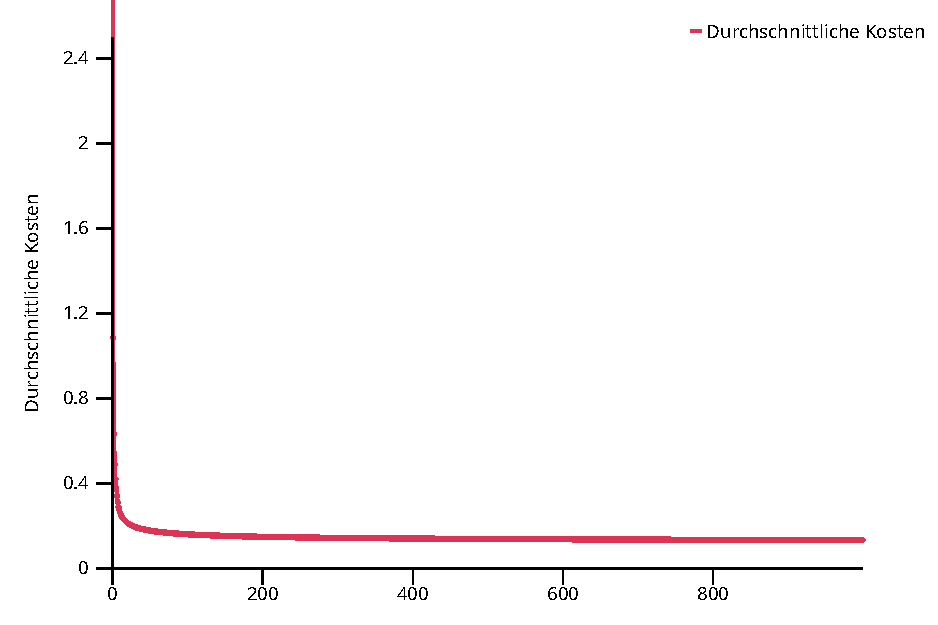
\includegraphics[width=\textwidth]{grafiken/kosten_1000}
        \caption{Entwickelung der Kosten des Netzes während des Trainingsprozesses}
        \label{fig:kosten-diagramm}
    \end{subfigure}
    \begin{subfigure}{0.45\textwidth}
        \centering
        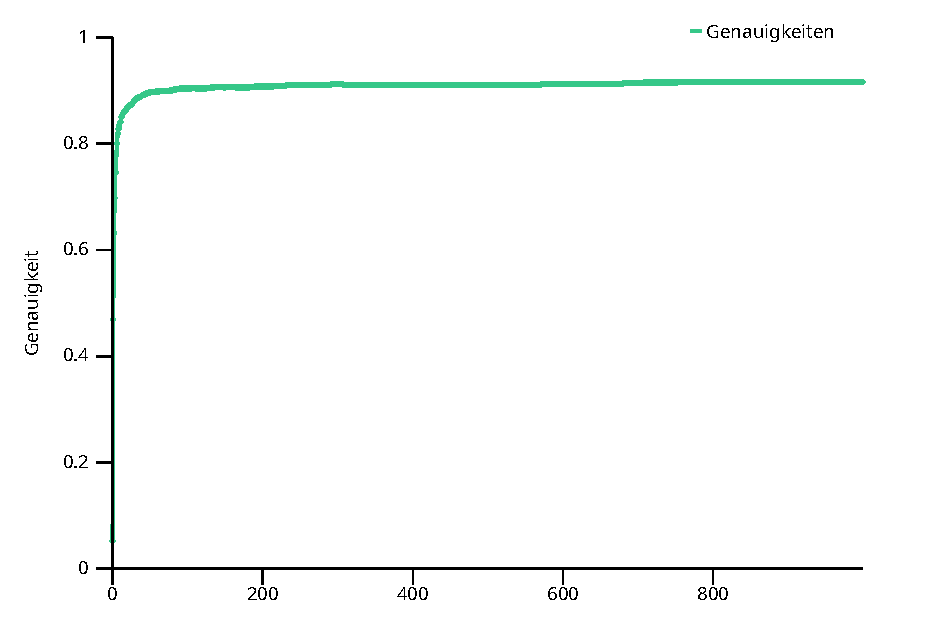
\includegraphics[width=\textwidth]{grafiken/genauigkeiten_1000}
        \caption{Entwickelung der Genauigkeiten des Netzes während des Trainingsprozesses}
        \label{fig:genauigkeiten-diagramm}
    \end{subfigure}
    \caption[Entwickelung der Kosten und Genauigkeiten während des Trainings: \textit{Eigene Grafik, erstellt mit plotlib für Rust}]{}
\end{figure}
    \pagebreak

    \section{Fazit}\label{sec:fazit}
In Rahmen dieser Facharbeit wurde die Funktionsweise von künstlichen neuronalen Netzen erklärt und in Form eines eigenen Programms implementiert.
Die eigene Implementierung kam dabei auf eine Genauigkeit von über 90\%, was ich für eine von Grund auf selbst implementierte Lösung für einen sehr guten Wert halte.
Das Ziel dieser Arbeit wurde somit erreicht.\\
Diese Arbeit beschäftigte sich ausschließlich mit einer Art von künstlichen neuronalen Netzen.
Um weitere, komplexere Arten von neuronalen Netzen verstehen zu können, ist es essenziell, das Gradientenverfahren, das \textit{Feedforward-Verfahren} und die Fehlerrückführung zu verstehen.
Weiterführend könnten die Themen Optimierungsverfahren für den Lernprozess oder die Architektur von KNN interessant sein.

    \section{Anhang}\label{sec:anhang}

\subsection{Literaturverzeichnis}\label{subsec:literaturverzeichnis}
\printbibliography[heading=none]

\subsection{Abbildungsverzeichnis}\label{subsec:abbildungsverzeichnis}
\lofwithouttitle

\subsection{Eigenständigkeitserklärung}\label{subsec:eigenstandigkeitserklarung}
Hiermit erkläre ich, dass ich diese Facharbeit ohne fremde Hilfe angefertigt habe und nur die im~\nameref{subsec:literaturverzeichnis} angegebenen Quellen und Hilfsmittel benutzt habe.\\
\linebreak
Hürth, 29.~März~2021\\
\includegraphics[height=1.2cm]{grafiken/unterschrift}

\end{document}
